% !TeX root = ../../script.tex
\documentclass[../../script.tex]{subfiles}

\begin{document}
\section{Contour Integrals}

\begin{defi}[Contour integrals]
    Let $U \subset \cmpln$ be open, $\gamma = C([a, b], U)$ a curve in $U$ and $f: U \rightarrow \cmpln$ continuous. Then 
    \[
        \int_{\gamma} f(z) \dd{z} := \int_a^b f(\gamma(t)) \gamma'(t) \dd{t}
    \]
\end{defi}

\begin{eg}
    Consider the path 
    \[
        \gamma(t) = re^{it}, ~\quad t \in [0, 2\pi], r > 0
    \]
    we want to take the contout integral along the path $\gamma$ of the function $z^n$
    \begin{align*}
        \int_{\gamma} z^n \dd{z} &= \int_0^{2\pi} (r e^{it})^n ire^{it} \dd{t}\\
        &= ir^{n+1} \int_0^{2\pi} e^{it(n+1)} \dd{t} = ir^{n+1} \begin{cases}
            2\pi, & n = -1 \\
            0, & n \ne -1
        \end{cases} 
    \end{align*}
\end{eg}

\begin{lem}[Estimation Lemma]
    For every curve $\gamma \in C([0, 1], U)$ and every continuous function $f: U \rightarrow \cmpln$ we have 
    \[
        \abs{\int_{\gamma} f(z) \dd{z}} \le \sup_{z \in \gamma} \abs{f(z)} \int_0^1 \abs{\gamma'(t)} \dd{t}
    \]
\end{lem}
\begin{proof}
    \begin{equation}
        \begin{split}
            \abs{\int_{\gamma} f(z) \dd{z}} = \abs{\int_0^1 f(\gamma(t)) \gamma'(t) \dd{t}} &\le \int_0^1 \abs{f(\gamma(t))} \abs{\gamma'(t)} \dd{t} \\
            &\le \sup_{t \in [0, 1]} \abs{f(\gamma(t))} \int_0^1 \abs{\gamma'(t)} \dd{t}
        \end{split}
    \end{equation}
\end{proof}

\begin{cor}
    Let $\gamma \in C([0, 1], U)$ be a simple closed curve, $U \subset \cmpln$, and let $f: U \rightarrow \cmpln$ a holomorphic function with 
    \begin{align*}
        u = \Re f && v = \Im f
    \end{align*}
    Then 
    \[
        \oint_{\gamma} f(z) \dd{z} = 0
    \]
\end{cor}
\begin{proof}
    Let $A \subset U$ be the surface bounded by $\gamma$. Then 
    \begin{equation}
        \oint_{\gamma} f(z) \dd{z} = \int_0^1 f(\gamma(t)) \gamma'(t) \dd{t}
    \end{equation}
    We can split $\gamma$ into a real and an imaginary part, like this 
    \begin{equation}
        \gamma(t) = \gamma_1(t) + i\gamma_2(t), \quad \gamma_1, \gamma_2: [0, 1] \rightarrow \realn
    \end{equation}
    Then we can calculate 
    \begin{equation}
        \begin{split}
            \oint_{\gamma} f(z) \dd{z} &= \int_0^1 \left(u(\gamma_1(t), \gamma_2(t)) + iv(\gamma_1(t), \gamma_2(t)) (\gamma_1'(t) + i\gamma_2'(t))\right) \dd{t} \\
            &= \int_0^1 u(\gamma_1(t), \gamma_2(t)) \gamma_1'(t) - v(\gamma_1(t), \gamma_2(t)) \gamma_2'(t) \dd{t} \\
            &\quad + i\int_0^1 u(\gamma_1(t), \gamma_2(t))\gamma_2'(t) + v(\gamma_1(t), \gamma_2(t))\gamma_1'(t) \dd{t} \\
            &= \int_0^1 \begin{pmatrix}
                u(\gamma(t)) \\ -v(\gamma(t))
            \end{pmatrix}
            \begin{pmatrix}
                \gamma_1'(t) \\ \gamma_2'(t)
            \end{pmatrix}
            \dd{t} + i \int_0^1 \begin{pmatrix}
                v(\gamma(t)) \\ u(\gamma(t))
            \end{pmatrix}
            \begin{pmatrix}
                \gamma_1'(t) \\ \gamma_2'(t)
            \end{pmatrix}
            \dd{t} \\
            &= \oint_{\boundary{A}} \begin{pmatrix}
                u \\ -v
            \end{pmatrix} \dd{s} + i \oint_{\boundary{A}} \begin{pmatrix}
                v \\ u
            \end{pmatrix} \\
            &= \int_A (-\partial_x v - \partial_y u) \dd{\lambda^2} + i \int_A (\partial_x u - \partial_y v) \dd{\lambda^2} \\
        \end{split}
    \end{equation}
    Because $f$ is holomorphic we can apply the Cauchy-Riemann equation 
    \begin{equation}
        \oint_{\gamma} f(z) \dd{z} = 0
    \end{equation}
\end{proof}

\begin{defi}
    \begin{enumerate}[(i)]
        \item A closed curve $\gamma: [a, b] \rightarrow U$ with $U \subset \cmpln$ is said to be null-homotopic,  
        if it can be continuously deformed into a point within the set $U$.

        \item Two curves $\gamma_1, \gamma_2: [0, 1] \rightarrow U$ with identical boundary points
        \begin{align*}
            \gamma_1(0) = \gamma_2(0) ~\wedge~ \gamma_1(1) = \gamma_2(1)
        \end{align*}
        is said to be homotopic in $U$ if the concatenation
        \begin{align*}
            \gamma: [0, 2] &\longrightarrow U \\
            \gamma(t) &= \begin{cases}
                \gamma_1(t), & t \in [0, 1] \\
                \gamma_2(2 - t) & t \in [1, 2]
            \end{cases}
        \end{align*}
        is null-homotopic.

        \item Two closed surves $\gamma_0, \gamma_1$ are said to be free-homotopic in $U$ if they can be continuously transformed into each other.
    \end{enumerate}
\end{defi}

\begin{defi}
    A non-empty set $U \subset \cmpln$ is said to be 
    \begin{enumerate}[(i)]
        \item \textit{connected} if any two points in $U$ can be connected by a curve in $U$.
        \item \textit{simply connected} if $U$ is connected and every closed surve in $U$ is null-homotopic.
        \item a \textit{domain} if it is open and connected.
    \end{enumerate}
\end{defi}

\begin{thm}[Cauchy's Integral Theorem]
    Let $f: U \rightarrow \cmpln$ be holomorphic and $\gamma$ a closed, null-homotopic curve in $U \subset \cmpln$ open. Then 
    \[
        \oint_{\gamma} f(z) \dd{z} = 0
    \]
\end{thm}
\begin{proof}
    \noproof
\end{proof}

\begin{cor}
    \begin{enumerate}[(i)]
        \item Let $\gamma_1, \gamma_2$ be holomorphic curves with the same endpoints on the open set $U \subset \cmpln$. Then 
        \[
            \int_{\gamma_1} f(z) \dd{z} = \int_{\gamma_2} f(z) \dd{z}
        \]
        for all holomorphic $f: U \rightarrow \cmpln$.

        \item For $f: U \rightarrow \cmpln$ holomorphic, with $U \subset \cmpln$ open and simple connected. Then $\forall z_0 \in U$
        \[
            F(z) := \int_{z_0}^{z} f(\zeta) \dd{\zeta} = \int_{\gamma = \gamma_0} f(\zeta) \dd{\zeta}
        \]
        is a holomorphic anti-derivative of $f$, i.e. 
        \[
            F'(z) = f(z) \quad \forall z \in U
        \]
    \end{enumerate}
\end{cor}

\begin{proof}
    First we prove (i). The concatenation $\gamma := \gamma_1 \gamma_2$ is a null-homotopic curve, so together with the holomorphy of $f$ we can apply the Cauchy integral theorem 
    \begin{equation}
        \begin{split}
            0 = \oint_{\gamma} f(z) \dd{z} &= \int_0^2 f(\gamma(t)) \dot{\gamma}(t) \dd{t} \\
            &= \int_0^1 f(\gamma_1(t))\dot{\gamma_1}(t) \dd{t} - \int_1^2 f(\gamma_2(2 - t)) \dot{\gamma_2}(2 - t) \dd{t}
        \end{split}
    \end{equation}
    Substitute $s = 2 - t$ with $\dd{s} = -\dd{t}$:
    \begin{equation}
        \begin{split}
            &= \int_0^1 f(\gamma_1(t)) \dot{\gamma}(t) \dd{t} - \gamma_0^1 f(\gamma_2(s)) \dot{\gamma_2}(s) \dd{s} \\
            &= \int_{\gamma_1} f(z) \dd{z} - \int_{\gamma_2} f(z) \dd{z}
        \end{split}
    \end{equation}

    Now we prove (ii). According to (i), we have 
    \begin{equation}
        F(z + h) = F(z) + \int_{\gamma_{z+h, z}} f(z) \dd{z}
    \end{equation}
    We choose $\gamma_{z+h, z}$ to be a straight line, i.e.
    \begin{equation}
        \gamma_{z+h, z}(t) = t(z + h) + (1 - t)z, \quad t \in [0, 1]
    \end{equation}
    Then
    \begin{equation}
        \int_{\gamma_{z+h, z}} 1 \dd{\zeta} = \int_0^1 \dot{\gamma}(t) \dd{t} = h
    \end{equation}
    Thus follows
    \begin{equation}
        F(z + h) - F(z) = \int_{\gamma_{z + h, z}} f(\zeta) \dd{\zeta} \iff \frac{F(z+h) - F(z)}{h} = \frac{1}{h} \in f(\zeta) \dd{\zeta} 
    \end{equation}
    and therefore 
    \begin{equation}
        \begin{split}
            \left| \frac{F(z+h) - F(z)}{h} - f(z) \right| = &\left| \frac{1}{h} \int_{\gamma_{z+h, z}} f(\zeta) \dd{\zeta} - f(z) \right| \\
            = &\left| \frac{1}{h} \int_{\gamma_{z+h, z}} f(\zeta) - f(z) \dd{\zeta} \right| \\
            = &\frac{1}{\abs{h}} \int_0^1 \left| f(\gamma_{z+h, z}(t)) - f(z)\right| \left| \dot{\gamma_{z+h, z}}(t) \right| \dd{t} \\
            \le &\frac{1}{h} \sup_{t \in [0, 1]} \left| f(\gamma_{z+h,z}(t)) - f(z) \right| \cdot \underbrace{\int \left| \dot{\gamma_{z+h, z}}(t) \right| \dd{t}}_{\abs{h}} \\
            = &\sup_{t \in [0, 1]} \left| f(\gamma_{z+h, z}(t)) - f(z) \right| \\
            \conv{k \rightarrow 0} &0
        \end{split}
    \end{equation}
\end{proof}

\begin{eg}[The complex logarithm]
    Consider $t \mapsto e^{it}, ~t \in \realn$. This is a $2\pi$-periodic function, that means
    \[
        e^{it} = e^{i(t + 2\pi n)}, \quad n \in \intn
    \]
    The function 
    \begin{align*}
        f: \cmpln \setminus \set{0} &\longrightarrow \cmpln \\
        z &\longmapsto \frac{1}{z}
    \end{align*}
    is holomorphic, and does not have an anti-derivative on $\cmpln \setminus \set{0}$. If it did, then 
    \[
        \int_{\gamma} f(z) \dd{z} = F(\gamma(2\pi)) - F(\gamma(0)) = 0
    \]
    would have to hold, but we know that 
    \[
        \int_{\gamma} \frac{\dd{z}}{z} = 2\pi i
    \]
    This is a contradiction. However $f$ does have an anti-derivative on $\cmpln_{-}$ (the complex numbers without the negative real axis) , since $\cmpln_{-}$ is simple connected and $f$ is holomorphic.
    Thus we can define 
    \begin{align*}
        \Log: \cmpln_{-} &\longrightarrow \cmpln \\
        z &\longmapsto \int_{\gamma: [0, 1] \rightarrow z} \frac{\dd{\zeta}}{\zeta}
    \end{align*}
    It can also be defined as 
    \begin{align*}
        \Log z = \begin{cases}
            0, & 1 \\
            \log\abs{z} + i \arg(z), & \text{else}
        \end{cases}
    \end{align*}
    The function $\arg$ is defined as 
    \begin{align*}
        \arg: \cmpln_{-} &\longrightarrow (-\pi, \pi) \\
        z &\longmapsto \phi \text{ for } z = \abs{z} e^{i\phi}
    \end{align*}
    $\Log$ is said to be the main branch of the complex logarithm, and 
    \[
        \Log z = \log\abs{z} + i (\arg(z) + 2\pi n), \quad n \in \intn
    \]
    the secondary branches.
\end{eg}

\begin{eg}[Fresnel Integrals]
    Consider the integrals 
    \begin{align*}
        \int_0^{\infty} \cos(t^2) \dd{t} && \int_0^{\infty} \sin(t^2) \dd{t}
    \end{align*}
    The way these integrals are supposed to be interpreted is as 
    \[
        \int_0^{\infty} f(t) \dd{t} = \lim_{N \rightarrow \infty} \int_0^N f(t) \dd{t}
    \]
    We realize that
    \begin{align*}
        \cos(t^2) = \Re e^{-it^2} && \sin(t^2) = -\Im e^{-it^2}
    \end{align*}
    Now, consider these paths
    \begin{center}
        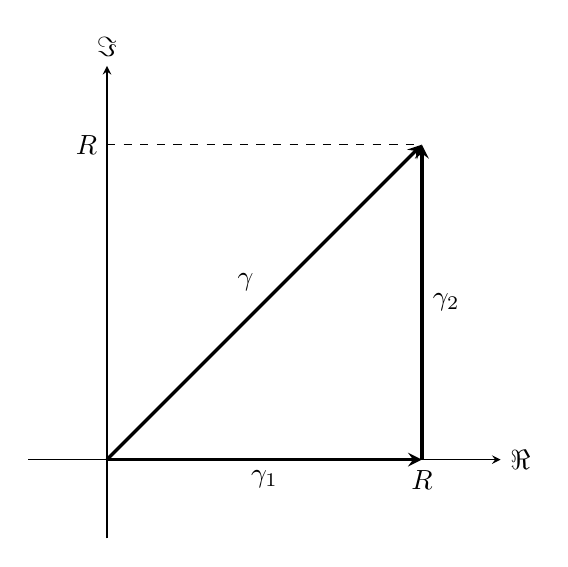
\begin{tikzpicture}
            \draw[->, >=stealth] (0, -1) -- (0, 5) node[above] {$\Im$};
            \draw[->, >=stealth] (-1, 0) -- (5, 0) node[right] {$\Re$};

            \draw[->, >=stealth, very thick] (0, 0) -- node[below] {$\gamma_1$} (4, 0) node[below] {$R$};
            \draw[->, >=stealth, very thick] (4, 0) -- node[right] {$\gamma_2$} (4, 4); 

            \draw[->, >=stealth, very thick] (0, 0) -- node[above left] {$\gamma$} (4, 4);

            \draw[dashed] (0, 4) node[left] {$R$} -- (4, 4);
        \end{tikzpicture}
    \end{center}
    So it becomes apparent that 
    \[
        \int_0^R \cos(t^2) \dd{t} = \Re \int_0^R e^{-it^2} \dd{t} = \Re \int_{\gamma} e^{-z^2} \dd{z}
    \]
    We can define a new (closed) path 
    \[
        \Gamma = \gamma_1 \gamma_2 (-\gamma)
    \]
    and with Cauchy's theorem we can realize that 
    \begin{align*}
        0 = \oint_{\Gamma} e^{-z^2} \dd{z} = \int_{\gamma_1} e^{-z^2} \dd{z} + \int_{\gamma_2} e^{-z^2} \dd{z} - \int_{\gamma} e^{-z^2} \dd{z}
    \end{align*}
    The next step is to evaluate each of the integrals in the last term, starting with the integral over $\gamma$.
    \begin{align*}
        \int_{\gamma} e^{-z^2} \dd{z} = &\int_0^R e^{-((1+i)t)^2} (1+i) \dd{t} \\
        = &(1 + i) \int_0^R e^{-2it^2} \dd{t} \\
        = &\frac{1+i}{\sqrt{2}} \int_0^{\sqrt{2} R} e^{-is^2} \dd{s}
    \end{align*}
    The integrall over $\gamma_1$ evaluates to 
    \begin{align*}
        \int_{\gamma_1} e^{-z^2} \dd{z} = \int_0^R e^{-t^2} \dd{t} \conv{R \rightarrow \infty} \int_0^{\infty} e^{-t^2} \dd{t} = \frac{1}{2} \int_{-\infty}^{\infty} e^{-t^2} \dd{t} = \frac{\sqrt{\pi}}{2}
    \end{align*}
    And the one over $\gamma_2$ to 
    \begin{align*}
        \int_{\gamma_2} e^{-z^2} \dd{z} = \int_0^R e^{-(r +it)^2} i \dd{t} = i \int_0^R e^{-R^2 + t^2} e^{-2irt} \dd{t}
    \end{align*}
    To evaluate this we need to consider the absolute value of this integral 
    \begin{align*}
        \abs{\int_{\gamma_2} e^{-z^2} \dd{z}} \le &e^{-R^2} \int_0^R e^{t^2} \underbrace{\abs{e^{-2iRt}}}_{=1} \dd{t} \\
        = &e^{-R^2} \int_0^R e^{t^2} \dd{t} \le e^{-R^2} \int_0^R e^{tR} \dd{t} \\
        = &e^{-R^2} \left[\frac{1}{R} e^{tR}\right]_0^R = \frac{e^{-R^2}}{R} \left(e^{R^2} - 1\right)
    \end{align*}
    so 
    \[
        \abs{\int_{\gamma_2} e^{-z^2} \dd{z}} \le \frac{1}{R} \left(1 - e^{-R^2}\right) \conv{R \rightarrow \infty} 0 
    \]
    Thus we can calculate 
    \[
        \int_{\gamma} e^{-z^2} \dd{z} = \frac{1+i}{\sqrt{2}} \int_0^{\sqrt{2} R} e^{-it^2} \dd{t} = \int_{\gamma_1} e^{-z^2} \dd{z} + \int_{\gamma_2} e^{-z^2} \dd{z}
    \]
    And finally 
    \begin{align*}
        \lim_{R \rightarrow \infty} \int_0^{\infty} e^{-it^2} \dd{t} = &\lim_{R \rightarrow \infty} \int_0^{\sqrt{2} R} e^{-t^2} \dd{t} \\
        = &\frac{\sqrt{2}}{1+i} \left(\lim_{R \rightarrow \infty} \left( \int_{\gamma_1} e^{-z^2} \dd{z} + \int_{\gamma_2} e^{-z^2} \dd{z} \right) \right) \\
        = &\frac{\sqrt{2}}{1+i} \left(\frac{\pi}{2} + 0\right) \\
        = &\sqrt{\frac{\pi}{2}} \frac{1-i}{2} = \sqrt{\frac{\pi}{8}} (1 - i)
    \end{align*}
    So we can calculate the Fresnel integrals
    \begin{align*}
        \int_0^{\infty} \cos(t^2) \dd{t} &= \sqrt{\frac{\pi}{8}} \\ 
        \int_0^{\infty} \sin(t^2) \dd{t} &= \sqrt{\frac{\pi}{8}} 
    \end{align*}
\end{eg}

\begin{thm}[Cauchy's Theorem for circular disks]
    Let $f: U \rightarrow \cmpln$ be holomorphic, $U \subset \cmpln$ open and $\cball[r](a) \subset U$. Then 
    \[
        f(a) = \frac{1}{2\pi i} \int_{\abs{z - a} = r} \frac{f(z)}{z-a} \dd{z}
    \]
\end{thm}
\begin{proof}
    Consider the following path
    \begin{center}
        \begin{tikzpicture}[scale=7.5]
            \draw[fill] (5, 0.7) node[below] {$a$} circle [radius=0.004];

            \begin{scope}[decoration={
                markings,
                mark=at position 0.5 with {\arrow{latex}}}
                ]
                \draw[thick, postaction={decorate}, domain=435:105] plot ({0.1*cos(\x) + 5}, {0.1*sin(\x) + 0.7}); 
                \draw[postaction={decorate}, domain=435:105] plot ({0.3*cos(\x) + 5}, {0.3*sin(\x) + 0.7});
                \draw[thick, postaction={decorate}] ({0.1*cos(105) + 5}, {0.1*sin(105) + 0.7}) -- node[left] {$\alpha_{\delta}^1$} ({0.3*cos(105) + 5}, {0.3*sin(105) + 0.7});
                \draw[thick, postaction={decorate}] ({0.3*cos(435) + 5}, {0.3*sin(435) + 0.7}) -- node[right] {$\alpha_{\delta}^2$} ({0.1*cos(435) + 5}, {0.1*sin(435) + 0.7});
                
                \draw[thick, postaction={decorate}, domain=105:75] plot ({0.3*cos(\x) + 5}, {0.3*sin(\x) + 0.7});
            \end{scope}

            \node[below] at ({0.1*cos(270) + 5}, {0.1*sin(270) + 0.7}) {$\gamma_{\epsilon}$};
            \node[below] at ({0.3*cos(270) + 5}, {0.3*sin(270) + 0.7}) {$|z - a| = r$};

            \draw[dashed] (5, 0.7) -- ({0.1*cos(150) + 5}, {0.1*sin(150) + 0.7}) node[above left=-0.1cm] {$\epsilon$} ;
            \draw[dashed] (5, 0.7) -- ({0.3*cos(5) + 5}, {0.3*sin(5) + 0.7}) node[right] {$r$};

            \node[above] at ({0.3*cos(90) + 5}, {0.3*sin(90) + 0.7}) {$\gamma_{\delta}$};
        \end{tikzpicture}
    \end{center}
    According to the first corollary of Cauchy's theorem we have
    \begin{equation}
    \begin{split}
        \int_{\abs{z-a}=r} \frac{f(z)}{z-a} \dd{z} = &\lim_{\delta \rightarrow 0} \int_{\gamma_{\epsilon, \delta}} \frac{f(z)}{z-a} \dd{z} + \underbrace{\int_{\alpha_{\delta}^1} \frac{f(z)}{z-a} \dd{z} + \int_{\alpha_{\delta}^2} \frac{f(z)}{z-a} \dd{z}}_{\conv{\delta \rightarrow 0} 0} \\
        = &\int_{\gamma_{\epsilon}} \frac{f(z)}{z-a} \dd{z}
    \end{split}
    \end{equation}
    Thus we conclude
    \begin{equation}
    \begin{split}
        \int_{\abs{z-a}=r} \frac{f(z)}{z-a} \dd{z} = \int_{\gamma_{\epsilon}} \frac{f(z)}{z-a} \dd{z} = &\int_{\gamma_{\epsilon}} \frac{f(z) - f(a)}{z-a} \dd{z} + \int_{\gamma_{\epsilon}} \frac{f(a)}{z-a} \dd{z} \\
        = &\int_{\gamma_{\epsilon}} \frac{f(z) - f(a)}{z-a} \dd{z} + f(a) \int_{\gamma_{\epsilon}} \frac{\dd{z}}{z-a}
    \end{split}
    \end{equation}
    We also know that 
    \begin{equation}
        \int_{\gamma_{\epsilon}} \frac{\dd{z}}{z-a} = 2\pi i
    \end{equation}
    Since $f$ is holomorphic we can realize
    \begin{equation}
        \sup_{\cball[r](a)} \left| \frac{f(z) - f(a)}{z - a} \right| = M_r < \infty
    \end{equation}
    Which results in 
    \begin{equation}
        \abs{\int_{\gamma_{\epsilon}} \frac{f(z) - f(a)}{z - a} \dd{z}} \le M_r \underbrace{\int_0^{2\pi} \abs{\dot{\gamma_{\epsilon}}(t)} \dd{t}}_{2\pi\epsilon} \conv{\epsilon \rightarrow 0} 0
    \end{equation}
    Thus follows 
    \begin{equation}
        \int_{|z - a| = r} \frac{f(z)}{z - a} \dd{z} = \int_{\gamma_{\epsilon}} \frac{f(z) - f(a)}{z - a} \dd{z} + 2\pi i f(a) \conv{\epsilon \rightarrow 0} 2\pi i f(a)
    \end{equation}
    Or short 
    \begin{equation}
        \int_{\abs{z - a} = r} \frac{f(z)}{z - a} \dd{z} = 2\pi i f(a)
    \end{equation}
\end{proof}

\begin{cor}
    Let $f: U \rightarrow \cmpln$ be a holomorphic function and $U \subset \cmpln$ an open set such that $\cball[r](a) \subset U$. Then 
    \[
        f(a) = \frac{1}{2\pi} \int_0^{2\pi} f(a + re^{it}) \dd{t}
    \]
\end{cor}
\begin{proof}
    \reader
\end{proof}

\begin{defi}[Analytic functions]
    Let $f: U \rightarrow \cmpln$ be a function and $U \subset \cmpln$ a domain. $f$ is said to be analytic in $z_0 \in U$ if and only if there exists a power series
    \[
        \sum_{n=0}^{\infty} a_n \zeta^n
    \]
    with convergence radius 
    \[
        \rho = \left(\limsup |a_n|^{\frac{1}{n}}\right)^{-1} > 0
    \]
    and $\delta \in (0, \rho)$ such that $\oball[\delta](z_0) \subset U$ and
    \[
        f(z) = \int_{k=0}^{\infty} a_n (z - z_0)^n, \quad \forall z \in \oball[\delta](z_0)
    \]
    $f$ is said to be analytic on $U$ if $f$ is analytic $\forall z_0 \in U$.
\end{defi}

\begin{thm}[Power series expansion]
    If $f$ is holomorphic on a circular disk $\oball[r](z_0)$ for some $r > 0$, then $f$ is analytic in $z_0$.
    $f$ can be represented with the on $\oball[\rho](z_0)$ convergent power series 
    \[
        f(z) = \sum_{n=0}^{\infty} c_n (z - z_0)^n, \quad z \in \oball[\rho](z_0)
    \]
    with 
    \[
        c_n = \frac{1}{2\pi i} \int_{|z - z_0| = r} \frac{f(z)}{(z - z_0)^{n+1}} \dd{z}, \quad \forall \rho \in (0, r)
    \]
\end{thm}
\begin{proof}
    \noproof
\end{proof}

\begin{rem}
    If $f$ is holomorphic then $f$ can be infinitely often differentiated on $\cmpln$ with 
    \[
        f^{(n)}(z) = n! c_n = \frac{n!}{2\pi i} \int_{\abs{z - z_0} = \rho} \frac{f(z)}{(z- z_0)^{n+1}} \dd{z}
    \]
    By employing the estimation lemma we can then find that 
    \begin{align*}
        \abs{c_n} \le \frac{1}{2\pi} \abs{\int_{\abs{z - z_0} = \rho} \frac{f(z)}{(z - z_0)^{n+1}} \dd{z}} \le &\frac{1}{2\pi} \sup_{\abs{z - z_0} = \rho} \abs{\frac{f(z)}{\abs{z - z_0}^{n+1}}} \cdot 2\pi \rho \\
        = &\frac{1}{\rho^n} \sup_{z \in \oball[r](z_0)} \abs{f(z)} \\
        = &\frac{M_r}{\rho^n}, \quad M_r < \infty
    \end{align*}
    This is Cauchy's estimate.
\end{rem}

\begin{thm}[Liouville's Theorem]
    Every bounded entire function is constant.
\end{thm}
\begin{proof}
    According to the power series expansion theorem, $f$ can be represented by a power series on all of $\cmpln$:
    \begin{equation}
        f(z) = \sum_{n=0}^{\infty} c_n z^n
    \end{equation}
    and the coefficients satisfy the Cauchy estimate
    \begin{equation}
        \abs{c_n} \le \frac{1}{\rho^n} \sup_{\abs{z} = \rho} \abs{f(z)} \le \frac{1}{\rho^n} \underbrace{\sup_{z \in \cmpln} \abs{f(z)}}_{< \infty}
    \end{equation}
    This inequality tends to $0$ if $\rho$ tends to $\infty$ for all $n \ge 1$, thus we can find 
    \begin{equation}
        c_n = 0, \quad \forall n \ge 1
    \end{equation}
    Thus 
    \begin{equation}
        f(z) = c_0 = \const.
    \end{equation}
\end{proof}

\begin{thm}[Fundamental Theorem of Algebra]\label{thm:fundamental}
    Every polynomial of degree $n \ge 1$
    \[
        f(z) = \sum_{k=0}^n c_k z^k, \quad c_n \ne 0
    \]
    has a root, i.e. 
    \[
        \exists z_0 \in \cmpln: \quad f(z_0) = 0
    \]
\end{thm}
\begin{proof}
    Assume there exists no root. Then the function 
    \begin{equation}
        z \longmapsto \frac{1}{f(z)}
    \end{equation}
    would be holomorphic on all of $\cmpln$, since $z \mapsto \rec{z}$ is holomorphic on $\cmpln \setminus \set{0}$.
    Furthermore we find that 
    \begin{equation}
        \exists R \ge 0: ~~\abs{z} \ge R \implies \abs{f(z)} \ge \abs{f(0)} > 0
    \end{equation}
    which implies 
    \begin{equation}
        \sup_{z \in \cmpln} \frac{1}{\abs{f(z)}} = \sup_{\abs{z} < R} \frac{1}{\abs{f(z)}} = \max_{\abs{z} \le R} \frac{1}{\abs{f(z)}} < \infty
    \end{equation}
    since $f$ doesn't have a root. According to Liouville's theorem $\rec{f}$ has to be constant, and thus $f$ must be constant. 
    This implies that $c_n = 0$, which contradicts the assumption. So $f$ has to have a root.
\end{proof}

\begin{cor}[Polynomial Decomposition]
    Let 
    \[
        f(z) = \sum_{k=0}^n c_k z^k, \quad n \in \natn, c_k \in \cmpln, c_n = 1
    \]
    Then $\exists z_j \in \cmpln, ~~j = 1, \cdots, n$ such that 
    \[
        f(z) = \prod_{j=1}^n (z - z_j)
    \]
\end{cor}
\end{document}